\documentclass[11pt,letterpaper]{article}
\usepackage[lmargin=1in,rmargin=1in,tmargin=1in,bmargin=1in]{geometry}
\usepackage{../style/homework}
\usepackage{../style/commands}
\setbool{quotetype}{false} % True: Side; False: Under
\setbool{hideans}{true} % Student: True; Instructor: False

% -------------------
% Content
% -------------------
\begin{document}

\homework{8: Due 10/13}{The difference between mathematicians and physicists is that after physicists prove a big result they think it is fantastic but after mathematicians prove a big result they think it is trivial.}{Lucien Szpiro}

% Problem 1
\problem{10} Consider the relation $f(x)$ given below. 
	\[
	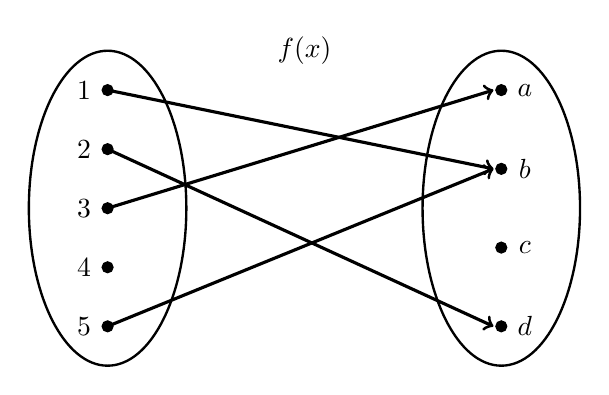
\begin{tikzpicture}
	\node at (2.5,2) {$f(x)$};
	% Ellipses
	\draw[line width=0.03cm] (0,0) circle (1 and 2);
	\draw[line width=0.03cm] (5,0) circle (1 and 2);
	
	% Nodes
	\draw[fill=black] (0,1.5) circle (0.07);
	\draw[fill=black] (0,0.75) circle (0.07);
	\draw[fill=black] (0,0) circle (0.07);
	\draw[fill=black] (0,-0.75) circle (0.07);
	\draw[fill=black] (0,-1.5) circle (0.07);
	
	\draw[fill=black] (5,1.5) circle (0.07);
	\draw[fill=black] (5,0.50) circle (0.07);
	\draw[fill=black] (5,-0.5) circle (0.07);
	\draw[fill=black] (5,-1.5) circle (0.07);
	
	
	% Arrow
	\draw[line width=0.04cm,->] (0,1.5) -- (4.9,0.50);
	\draw[line width=0.04cm,->] (0,0.75) -- (4.9,-1.5);
	\draw[line width=0.04cm,->] (0,0) -- (4.9,1.5);
	\draw[line width=0.04cm,->] (0,-1.5) -- (4.9,0.5);

	
	% Labels
	\node at (-0.3,1.5) {$1$};
	\node at (-0.3,0.75) {$2$};
	\node at (-0.3,0) {$3$};
	\node at (-0.3,-0.75) {$4$};
	\node at (-0.3,-1.5) {$5$};
	
	\node at (5.3,1.5) {$a$};
	\node at (5.3,0.5) {$b$};
	\node at (5.3,-0.5) {$c$};
	\node at (5.3,-1.5) {$d$};
	\end{tikzpicture}
	\]

\begin{enumerate}[(a)]
\item Explain why $f(x)$ is not a function. 
\item Add an arrow to the diagram so that $f(x)$ is a surjective function.
\item Identify the domain, codomain, and range for $f(x)$. 
\item Is $f(x)$ an injective function? Explain why or why not. 
\end{enumerate}



\newpage



% Problem 2
\problem{10} Complete the proof of the proposition stated below by filling in the blanks. \pspace

\noindent {\bfseries Proposition.} Let $f: X \to Y$ be a function and $B \subseteq Y$. Then $X \setminus f^{-1}(B) \subseteq f^{-1}(Y \setminus B)$. \pspace

\noindent {\itshape Proof.} We know that if $X \setminus f^{-1}(B)= \varnothing$, then $X \setminus f^{-1}(B) \subseteq f^{-1}(Y \setminus B)$. Assume that \pspace

$X \setminus f^{-1}(B)\neq \varnothing$. To show that $X \setminus f^{-1}(B) \subseteq f^{-1}(Y \setminus B)$, we need to show that if \underline{\hspace{3cm}}, \pspace

then \underline{\hspace{3cm}}. \pspace

Let $x \in X \setminus f^{-1}(B)$. But then we know that \underline{\hspace{3cm}} and $x \notin$ \underline{\hspace{3cm}}. Because \pspace

$x \notin$ \underline{\hspace{3cm}}, we know that $f(x) \notin$ \underline{\hspace{3cm}}. It is clear that $f(x) \in Y$. But then \pspace

\underline{\hspace{3cm}} and $f(x) \notin$ \underline{\hspace{3cm}}. This shows that $f(x) \in$ \underline{\hspace{3cm}}. \pspace

This shows that $f(x)$ is in the preimage of $Y \setminus B$. But then we know that $x \in$ \underline{\hspace{3cm}}. \pspace

But then if $x \in$ \underline{\hspace{3cm}}, then $x \in$ \underline{\hspace{3cm}}. Therefore, $X \setminus f^{-1}(B) \subseteq f^{-1}(Y \setminus B)$.



\newpage



% Problem 3
\problem{10} Let $f: \mathbb{R} \to \mathbb{R}$ be the function given by $x \mapsto x^2 + 3x - 7$. 
	\begin{enumerate}[(a)]
	\item Without referencing the graph of $f$, use the definition of decreasing to show that $f(x)$ is not a decreasing function on $\mathbb{R}$ by giving a counterexample. 
	\item Determine whether or not $3 \in \text{im } f$. If $3 \in \text{im } f$, find an element in the preimage of 3. If $3 \notin \text{im } f$, explain why. 
	\item Is $f^{-1}(x)$ a function? Explain why or why not by referencing the graph of $f(x)$. Give an additional explanation of why or why not using your response in (b). 
	\end{enumerate}


\end{document}